%%
%% This is file `sample-sigplan.tex',
%% generated with the docstrip utility.
%%
%% The original source files were:
%%
%% samples.dtx  (with options: `sigplan')
%% 
%% IMPORTANT NOTICE:
%% 
%% For the copyright see the source file.
%% 
%% Any modified versions of this file must be renamed
%% with new filenames distinct from sample-sigplan.tex.
%% 
%% For distribution of the original source see the terms
%% for copying and modification in the file samples.dtx.
%% 
%% This generated file may be distributed as long as the
%% original source files, as listed above, are part of the
%% same distribution. (The sources need not necessarily be
%% in the same archive or directory.)
%%
%% The first command in your LaTeX source must be the \documentclass command.
\documentclass[sigplan,screen]{acmart}

%%
%% \BibTeX command to typeset BibTeX logo in the docs
\AtBeginDocument{%
  \providecommand\BibTeX{{%
    \normalfont B\kern-0.5em{\scshape i\kern-0.25em b}\kern-0.8em\TeX}}}

%% Rights management information.  This information is sent to you
%% when you complete the rights form.  These commands have SAMPLE
%% values in them; it is your responsibility as an author to replace
%% the commands and values with those provided to you when you
%% complete the rights form.
\setcopyright{acmcopyright}
\copyrightyear{2020}
\acmYear{2020}
\acmDOI{10.1145/1122445.1122456}

%% These commands are for a PROCEEDINGS abstract or paper.
\acmConference[Woodstock '18]{Woodstock '18: ACM Symposium on Neural
  Gaze Detection}{June 03--05, 2018}{Woodstock, NY}
\acmBooktitle{Woodstock '18: ACM Symposium on Neural Gaze Detection,
  June 03--05, 2018, Woodstock, NY}
\acmPrice{15.00}
\acmISBN{978-1-4503-XXXX-X/18/06}

\usepackage[T2A]{fontenc}
\usepackage[utf8]{inputenc}

\usepackage[english,russian]{babel}
\usepackage{listings}
\usepackage[section]{placeins}
\usepackage{multirow}
\usepackage{pgfplots}
\usepackage{yfonts}
\usepackage{subcaption}
\usepackage{xspace}
% \usepackage{amssymb}
\usepackage{amsmath}
\usepackage{comment}
\usepackage{url}
\usepackage{tikz}
\usetikzlibrary{trees}

%\pgfplotsset{width=7cm,compat=1.8}

\lstdefinelanguage{ocanren}{
keywords={run, conde, fresh, let, in, match, with, when, class, type,
object, method, of, rec, until, while, not, do, done, as, val, inherit,
new, module, sig, deriving, datatype, struct, if, then, else, open, private, virtual, include, success, failure,
true, false},
sensitive=true,
commentstyle=\small\itshape\ttfamily,
keywordstyle=\textbf,%\ttfamily\underline,
identifierstyle=\ttfamily,
basewidth={0.5em,0.5em},
columns=fixed,
mathescape=true,
fontadjust=true,
literate={fun}{{$\lambda$}}1 {->}{{$\to$}}3 {===}{{$\equiv$}}1 {=/=}{{$\not\equiv$}}1 {|>}{{$\triangleright$}}3 {\\/}{{$\vee$}}2 {/\\}{{$\wedge$}}2 {^}{{$\uparrow$}}1,
morecomment=[s]{(*}{*)} %,
%numbers=left
}

\lstset{
language=ocanren
}

\newcommand{\ruleno}[1]{\mbox{[\textsc{#1}]}}
\newcommand{\rulen}[1]{[\textsc{#1}]}
\newcommand{\mk}{\textsc{miniKanren}\xspace}
\newcommand{\inbr}[1]{\langle #1 \rangle}
\renewcommand{\emptyset}{\varnothing}
\newcommand{\primi}[1]{\mbox{\bf #1}}

%%
%% Submission ID.
%% Use this when submitting an article to a sponsored event. You'll
%% receive a unique submission ID from the organizers
%% of the event, and this ID should be used as the parameter to this command.
%%\acmSubmissionID{123-A56-BU3}

%%
%% The majority of ACM publications use numbered citations and
%% references.  The command \citestyle{authoryear} switches to the
%% "author year" style.
%%
%% If you are preparing content for an event
%% sponsored by ACM SIGGRAPH, you must use the "author year" style of
%% citations and references.
%% Uncommenting
%% the next command will enable that style.
%%\citestyle{acmauthoryear}

%%
%% end of the preamble, start of the body of the document source.
\sloppy
\begin{document}

%%
%% The "title" command has an optional parameter,
%% allowing the author to define a "short title" to be used in page headers.
\title{Efficient Fair Conjunction for\\
  Structurally-Recursive Relations}

%%
%% The "author" command and its associated commands are used to define
%% the authors and their affiliations.
%% Of note is the shared affiliation of the first two authors, and the
%% "authornote" and "authornotemark" commands
%% used to denote shared contribution to the research.
\author{Peter Lozov}
%\authornote{Both authors contributed equally to this research.}
\email{lozov.peter@gmail.com}
\orcid{0000-0003-3563-2828}
\author{Dmitry Boulytchev}
%\authornotemark[1]
\email{dboulytchev@math.spbu.ru}
\orcid{0000-0001-8363-7143}
\affiliation{%
  \institution{St.Petersburg State University, JetBrains Research}
  \streetaddress{P.O. Box 1212}
  \city{St.Petersburg}
  \country{Russia}
  \postcode{43017-6221}
}
%%
%% By default, the full list of authors will be used in the page
%% headers. Often, this list is too long, and will overlap
%% other information printed in the page headers. This command allows
%% the author to define a more concise list
%% of authors' names for this purpose.
\renewcommand{\shortauthors}{Lozov and Boulytchev}

%%
%% The abstract is a short summary of the work to be presented in the
%% article.
\begin{abstract}
  We present a new, \emph{fair}, conjunction evaluation strategy for relational programming languge \mk. Unlike the original left-biased
  conjunction, our approach controls the order of conjunct execution based on the intrinsic properties of relation definitions.
  We present both the formal study of conjunction fairness and practical evaluation, which demonstrates the essential
  improvement in terms of both performance and convergence.
\end{abstract}

%%
%% The code below is generated by the tool at http://dl.acm.org/ccs.cfm.
%% Please copy and paste the code instead of the example below.
%%
\begin{CCSXML}
<ccs2012>
<concept>
<concept_id>10003752.10010124.10010131.10010134</concept_id>
<concept_desc>Theory of computation~Operational semantics</concept_desc>
<concept_significance>500</concept_significance>
</concept>
<concept>
<concept_id>10003752.10003790.10003795</concept_id>
<concept_desc>Theory of computation~Constraint and logic programming</concept_desc>
<concept_significance>500</concept_significance>
</concept>
</ccs2012>
\end{CCSXML}

\ccsdesc[500]{Theory of computation~Operational semantics}
\ccsdesc[500]{Theory of computation~Constraint and logic programming}

%%
%% Keywords. The author(s) should pick words that accurately describe
%% the work being presented. Separate the keywords with commas.
\keywords{relational programming, miniKanren, evaluation strategies, operational semantics}

%% A "teaser" image appears between the author and affiliation
%% information and the body of the document, and typically spans the
%% page.
%\begin{teaserfigure}
%  \includegraphics[width=\textwidth]{sampleteaser}
%  \caption{Seattle Mariners at Spring Training, 2010.}
%  \Description{Enjoying the baseball game from the third-base
%  seats. Ichiro Suzuki preparing to bat.}
%  \label{fig:teaser}
%\end{teaserfigure}

%%
%% This command processes the author and affiliation and title
%% information and builds the first part of the formatted document.
\maketitle

\section{Introduction}
\label{sec:intro}

Algebraic data types (ADT) is an important tool in functional programming which delivers a way to represent flexible and easy to manipulate data structures.
To inspect the contents of ADT values a generic construct~--- \emph{pattern matching}~--- is used. Pattern matching can be considered as a generalization of
conventional conditional control-flow construct ``\lstinline|if .. then .. else|'' and in principle can be decomposed into a nested hierarchy of those; from
this standpoint the problem of pattern matching implementation can be considered trivial. However, some decompositions are obviously better than others. We
repeat here an example from~\cite{maranget2008} to demonstrate this difference (see Fig.~\ref{fig:match-example}). Here we match a triple of boolean
values $x$, $y$, and $z$ against four pattern (Fig.~\ref{fig:matching-example1}; we use \textsc{OCaml}~\cite{ocaml} as reference language). The na\"{i}ve
implementation of this example is shown on Fig.~\ref{fig:matching-example2}; however if we decide to match $y$ first the result becomes much
better (Fig.~\ref{fig:matching-example3}).

\begin{figure}[ht]
\begin{subfigure}[t]{0.2\linewidth}
\centering
\begin{lstlisting}
match x, y, z with
| _, F, T -> 1
| F, T, _ -> 2
| _, _, F -> 3
| _, _, T -> 4
\end{lstlisting}
\vskip18.5mm
\caption{Pattern matching}
\label{fig:matching-example1}
\end{subfigure}
\hspace{0.5cm}
\begin{subfigure}[t]{0.26\linewidth}
\centering
\begin{lstlisting}
if x then
  if y then
    if z then 4 else 3
  else
    if z then 1 else 3
else
  if y then 2
  else
    if z then 1 else 3
\end{lstlisting}
\caption{A correct but non-optimal\\\phantom{(b)~}implementation}
\label{fig:matching-example2}
\end{subfigure}
\hspace{0.5cm}
\begin{subfigure}[t]{0.33\linewidth}
\centering
\begin{lstlisting}
if y then
  if x then
    if z then 4 else 3
  else 2
else
  if z then 1 else 3
\end{lstlisting}
\vskip13.5mm
\caption{Optimal implementation}
\label{fig:matching-example3}
\end{subfigure}
\caption{Pattern matching implementation example} 
\label{fig:match-example}
\end{figure}

\begin{comment}
\begin{figure}[ht]
\begin{minipage}[b]{0.3\linewidth}
\centering
\label{fig:figure1}
\end{minipage}
\hspace{0.5cm}
\begin{minipage}[b]{0.3\linewidth}
\centering
\begin{lstlisting}
switch x with 
| true -> 
    switch y with 
    | true -> 
       switch z with 
       | true -> 4
       | _ -> 3
    | _ -> 
      switch z with 
      | true -> 1
      | _ -> 3 
| _ -> 
   switch y with 
   | true -> 2 
   | _ -> if z then 1 else 3
\end{lstlisting}
\end{minipage}
\hspace{0.5cm}
\begin{minipage}[b]{0.3\linewidth}
\centering
\end{minipage}
\end{figure}
\end{comment}


%clasification 1
Although semantics of pattern matching can be given as a sequence of srutinee's sub expression comparisons (Figure~\ref{fig:matchpatts}) effective compilers don't follow
this approach. One can either optimise runtime cost by minimizing amount of checks performed or static cost by minimizing the size of generated code. \emph{Decision trees}~\cite{?}
are good for the first criteria, because they check every subexpression not more than once. \emph{Backtracking automata} are rather compact but in some cases can perform
repeated checks.

%clasification 2
\emph{For strict languages} checking sub-expressions of scrutinee in any order is allowed. \emph{For lazy languages} pattern matching should evaluate only those sub-expressions which are
necessary for performing pattern matching. If not careful pattern matching can change the termination behavior of the program. In general lazy languages setup more constraints on pattern matching and because of that allow lesser set of heuristics. Decision trees and backtracking automata can be used for compilation both  strict and lazy languages.

%clasification 3
The matching compilers for strict languages can work in \emph{direct} or \emph{indirect} styles. The first ones return efficient code immediately. In the second style to
construct final answer some post processing is required. It can vary from easy simplifications to complicated supercompilation techniques~\cite{sestoft1996}. The main
drawback of indirect style is that the size of intermediate data structures can be exponentially large.

% about lazy languages
A few approaches for checking sub-expressions in lazy languages has been proposed. In ~\cite{augustsson1985} simple left-to-right order of subexpression checking was proposed and was proved that it doesn't affect termination. The backtracking automaton being built has a form of a DAG to reduce code size. A few refinements has been added by~\cite{wadler1987} as a part of textbook~\cite{peytonjones1987} about implementing lazy functional languages. The implementation from this book is being used in the current version of GHC~\cite{ghc}. \cite{laville1991} models values in lazy languages
using \emph{partial terms}, although it doesn't scale to types with infinite constructor sets (like integers). The approach doesn't test all subexpressions from left to right as~\cite{augustsson1985} but aims to not perform unnecessary check by constructing \emph{lazy automaton}. 
%In~\cite{suarez1993} the similar approach is extended by special treatment of overlapping patterns.

% about decision trees
Pattern matching for lazy languages has been compiled also to decision trees~\cite{maranget1992} and later (\cite{maranget1994}) into
\emph{decision DAGs} which allow in some cases to make code smaller.

Minimizing the size of decision tree is known to be NP-hard~\cite{baudinet1985tree}, and as a rule various heuristics are applied during compilation, for example, the number of nodes,
the length of the longest path, the average length of all paths. The paper~\cite{Scott2000WhenDM} performs experimental evaluation of nine heuristics on the base of for strict language Standard ML of New Jersey.

%about automata
The inefficiency of backtracking automaton has been
improved in~\cite{maranget2001}. The approach utilizes matrix representation for pattern matching. It splits the current matrix according to constructors in the
first column and reduces the task to compiling matrices with less rows. The technique is indirect, in the end a few optimizations are performed by introducing
special \emph{exit} nodes to the compiled representation. No preprocessing is required for this scheme: or-pattern receives a special treatment during compilation process.
The approach from this paper is used in the current implementation of the \textsc{OCaml} compiler.

Previous approach uses first column to split the matrix. In~\cite{maranget2008} the \emph{necessity} heuristic has been introduced which recommends which column should be
used to perform the split. Good decision trees which are constructed in this work can perform better on corner cases than~\cite{maranget2001}, but for practical cases the
difference is insignificant.


While existing approaches deliver appropriate solutions for certain forms of pattern matching construct, they have to be extended in an \emph{ad hoc} manner each time
the syntax and semantics of pattern matching construct changes. For example, besides a simple conventional form of pattern matching there is a number of extensions
(guards~\cite{?}, disjunctive patterns~\cite{?}, non-linear patterns~\cite{mcbride1969symbol}, active patterns~\cite{activepatterns}, pattern matching for polymorphic variants~\cite{Garrigue98} and generalized
algebraic datatypes~\cite{?}) which require a separate customized algorithms to be developed.

\begin{comment}
\begin{minipage}[b]{0.5\textwidth}
There are a few different approaches for compiling pattern mathcing. For example, \textsc{GHC}~\cite{?} uses that presented in an influential paper~\cite{Jones1987},
implementation of pattern matching in \textsc{OCaml} is currently based on~\cite{maranget2001} although \cite{maranget2008} reports a slight improvements
of generated code efficiency. 
\end{minipage}
\end{comment}

We present an approach to pattern matching implementation based on application of relational programming~\cite{TRS,WillThesis} and, in particular, relational interpreters~\cite{unified}
and relational conversion~\cite{lozov2017}. Our approach is based on relational representation of the top-level source language semantics of pattern matching on the one hand, and
the semantics of intermediate-level implementation language on the other. We formulate the condition for a correct and complete implementation of pattern matching and use it to
construct a top-level goal which represents a search procedure for all correct and complete implementations. We also present a number of techniques which makes it possible to come up with an
\emph{optimal} solution as well as optimizations to improve the performance of the search. Our implementation\footnote{\url{https://github.com/kakadu/pat-match}} makes use of
\textsc{OCanren}\footnote{\url{https://github.com/JetBrains-Research/OCanren}}~--- a typed implementation of \textsc{miniKanren} for \textsc{OCaml}~\cite{OCanren},
and \textsc{noCanren}\footnote{\url{https://github.com/Lozov-Petr/noCanren}}~--- a convertor from the subset of plain \textsc{OCaml} into \textsc{OCanren}~\cite{lozov2017}.
An evaluation, performed for a set of benchmarks taken from other papers, initially has shown a good performance of our synthesizer. However, being aware of some pitfalls of
our approach, we came up with a set of counterexamples, on which it did not provide any results in observable time, so we do not consider the problem completely solved.
We also started a work on mechanized formalization\footnote{\url{https://github.com/dboulytchev/Coq-matching-workout}}, written in \textsc{Coq}~\cite{Coq}, to
make the justification of out approach more solid and easier to verify, but this formalization is not yet complete. 

 

\section{Exposition: \mk and Biased Conjunction}
\label{sec:exposition}

In this section we give a formal syntax for the language we will use in the rest of the paper. We also describe the intentions and common design
choices lying behind existing implementations and demonstrate on a number of examples the ``biased conjunction problem'' which we are going to attack.
As the material of this section serves mainly as a motivation we will not present a formal semantics for the language, which can be found in~\cite{fair:semantics},
and leave out the description of some subtleties.

The syntax of the language is shown in Fig.~\ref{syntax}. We conventionally define the set of terms $\mathcal{T}_\mathcal{X}$
over the constructors with arities $\mathcal{C}$ and \emph{syntactic} variables $\mathcal{X}$. Note, we keep the parameterization of $\mathcal{T}_\mathcal{X}$ by $\mathcal{X}$
explicit since later we will also use another its parameterization by the set of \emph{semantic} variables. We also define the set $\mathcal{R}$ of relation names with arities.

Next, we introduce the central construct of \mk~--- a goal $\mathcal{G}$. A goal is either a unification of terms, disjunction or conjunction of goals, introduction of fresh variable,
or an application of a relation to terms. Relation definition $\mathcal{D}$ corresponds to an abstraction of a goal over the set of arguments. Finally, a specification $\mathcal{S}$
puts a top-level goal in the context of a list of relation definitions.

In a nutshell, here we deal with a simple first-order language in which goals play a role of function bodies and ``\lstinline|fresh|''~--- additional binders. Thus,
conventional notions of free variables and substitutions of variables by terms in terms and goals come naturally.

From now on we stipulate that all specifications are well-formed, meaning that all relational names have unique definitions, none of the definitions has
free variables and all relation applications respect the arity of corresponding relation names. The only place where free variables can be encountered in specification
is its top-level goal, and the evaluation of this goal delivers all bindings (\emph{answers}) for these variables which satisfy the constraints imposed by the specification.

More concretely, a goal defines a search procedure which for a given \emph{state} returns a finite or infinite stream of states. For now we can assume that states are represented by
substitutions from variables to terms although in actual implementations they can hold some extra information needed, for example, for allocating fresh variables.
This procedure is defined inductively by case analysis on the shape of the goal (we denote current substitution as $\theta$):

\begin{itemize}
\item For unification $t_1 \equiv t_2$ an attempt to unify the terms $t_1\theta$ and $t_2\theta$ is made. On success the most general unifier is integrated into $\theta$ and the resulting substitution
  is returned as a one-element stream; otherwise an empty stream in returned.

\item For disjunction $g_1 \vee g_2$ the evaluation steps of $g_1\,(\theta)$ and $g_2\,(\theta)$ are taken in an alternating manner, and the results are collected in a common stream. This evaluation
  discipline~--- \emph{interleaving}~\cite{fair:interleaving}~--- provides the \emph{completeness} of \mk search: each answer will be found in a finite number of steps.

\item For conjunction $g_1 \wedge g_2$, first, the left conjunct $g_1\,(\theta)$ is fully evaluated. Then, for each element $\theta^\prime$ (if any) of the resulting stream $g_2\,(\theta^\prime)$ is
  evaluated, and all resulting streams are concatenated. Thus, the evaluation of conjunction is \emph{left-biased}: none of evaluation steps in $g_2$ are performed until the next answer for
  $g_1\,(\theta)$ is found.

\item For fresh variable introduction \lstinline|fresh ($x$) $\;g$| a new variable, not occurring anywhere in $\theta$, is chosen and substituted for $x$ in $g$. Then the resulting goal is evaluated.

\item For relation application $R^k\,(t_1,\dots,t_k)$ the corresponding definition $R^k=\lambda x_1\dots x_k\,.\,g$ is found and all variables $x_i$ are substituted by terms $t_i$ in
  $g$. Then the resulting goal is evaluated for $\theta$ (we assume no capturing occurs during the substitution).
\end{itemize}

\begin{figure}[t]
\[
  \begin{array}{rcll}
     \mathcal{C} & = & \{ C_1^{k_1}, C_2^{k_2}, \ldots \} 
     & \mbox{constructors with arities} 
     \\
     \mathcal{X} & = & \{x_1, x_2, \ldots \} 
     & \mbox{syntactic variables} 
     \\
     \mathcal{T}_\mathcal{X} & = & \mathcal{X} \mid C_i^{k_i}(\mathcal{T}_\mathcal{X}^1, \ldots, \mathcal{T}_\mathcal{X}^{k_i})
     & \mbox{syntactic terms} 
     \\
     \mathcal{R} & = & \{R_1^{k_1}, R_2^{k_2}, \ldots \} 
     & \mbox{relation names} 
     \\
     \mathcal{G} & =    & \mathcal{T}_\mathcal{X} \equiv \mathcal{T}_\mathcal{X} & \mbox{unification} \\
                 & \mid & \mathcal{G} \lor \mathcal{G} & \mbox{disjunction} \\
                 & \mid & \mathcal{G} \land \mathcal{G} & \mbox{conjunction} \\
                 & \mid & \mbox{\lstinline|fresh|} \; (\mathcal{X}) \; \mathcal{G} & \mbox{fresh variable introduction} \\
                 & \mid & R_i^{k_i}(\mathcal{T}_\mathcal{X}^1, \ldots, \mathcal{T}_\mathcal{X}^{k_i}) & \mbox{relation application} \\
    \mathcal{D} & = &R_i^{k_i} = \lambda \mathcal{X}_1 \ldots \mathcal{X}_{k_i}. \; \mathcal{G} & \mbox{relation definition}\\
    \mathcal{S} & = &\mathcal{D}_1\mathcal{D}_2\dots\mathcal{D}_k \diamond \mathcal{G} & \mbox{specification}
  \end{array}
\]
    \caption{The syntax of relational language}
    \label{syntax}
\end{figure}


It is easy to see that this implementation ideas give rise to a monadic framework over the set of streams with evaluation rules for conjunction and disjunction playing roles of ``bind'' and
``mplus'' respectively. In an actual implementation a few embellishments can be added to this general framework: for example, some evaluation steps can be deferred using so-called
\emph{inverse-$\eta$-delay}~\cite{MicroKanren}; in conjunction instead of left conjunct the right one can be chosen for evaluation first; various interleaving disciplines can
be applied to make the distribution of steps within a cluster of disjunctions more fair~\cite{fair:towardsAM}, etc. However, in all cases the basic implementation principles remain
the same.

We now consider a few examples of relational definitions and specifications. The following definition\footnote{By tradition, the names of relations are superscripted by ``$^o$''.}
introduces a relational list concatenation:

\begin{lstlisting}
  append$^o$ = $\lambda\; x\; y\; xy$ . ($x$ ===$\,$ [] /\ $y$ === $\;xy$) \/
                      fresh ($e\; xs\; xys$) 
                        $x\;$ === $\;e$ : $xs$ /\ 
                        $xy\;$ === $\;e$ : $xys$ /\ 
                        append$^o$ $xs\; y\; xys$
\end{lstlisting}

Three arguments $x$, $y$ and $xy$ correspond to three lists such that the concatenation of $x$ and $y$ equals $xy$. The relation is defined using case analysis and recursion: if
$x$ is empty (\lstinline|[]|) then $xy$ should be equal $y$; otherwise we split $x$ into a head $e$ and a tail $xs$ and set $y$ to \lstinline|$e$ : $xys$|, where
$xys$ is a concatenation of $xs$ and $y$, obtained via a recursive call to the same relation (we use here ``\lstinline|[]|'' and ``\lstinline|:|'' as constructor names).

In the context of this definition the top-level goal

\begin{lstlisting}
       append$^o$ [A] [B] $x$
\end{lstlisting}

would calculate a substitution

\[
x \mapsto \mbox{\lstinline|[A, B]|}
\]

which is an expected outcome. However, as unification actually works in both direction, the same relation can be used to solve other problems as well. For example

\begin{lstlisting}
       append$^o$ [A] $x$ [A, B]
\end{lstlisting}

gives us

\[
x \mapsto \mbox{\lstinline|[B]|}
\]

while

\begin{lstlisting}
       append$^o$ $x$ $y$ [A, B]
\end{lstlisting}

gives us a whole bunch of answers

\[
\begin{array}{ll}
  x \mapsto \mbox{\lstinline|[]|} & y \mapsto \mbox{\lstinline|[A, B]|} \\
  x \mapsto \mbox{\lstinline|[A]|} & y \mapsto \mbox{\lstinline|[B]|} \\
  x \mapsto \mbox{\lstinline|[A, B]|} & y \mapsto \mbox{\lstinline|[]|} 
\end{array}
\]

(not necessarily in this order). In other words, the same relation definition can be used to perform the search in various ``directions''~--- not only calculate
outputs for given inputs, but also vice versa, and, generally in any possible way depending on the distribution of free variables.

In all aforementioned examples the evaluation of a goal returned a finite stream. This is, however, not always the case. For example, if we put the recursive call in the definition of
\lstinline|append$^o$| \emph{first} in the conjunction, then the evaluation of the goal \lstinline|append$^o$ $x$ $y$ [A, B]| will \emph{diverge} after returning all the answers. We
can illustrate this behavior by the following diagram:

\begin{tikzpicture}[sibling distance=3cm,edge from parent/.style={draw,-latex}]
  \node{\lstinline|append$^o$ $x$ $y$ [A, B]|}
    child {
      node{$\begin{array}{l}
              x\mapsto\mbox{\lstinline|[]|}\\
              y\mapsto\mbox{\lstinline|[A, B]|}
            \end{array}$}
    }
    child {
      node{\lstinline|append$^o\;$ $xs\;$ $y\;$ $xys$|}
        child {
          node{$\begin{array}{l}
                  xs\mapsto\mbox{\lstinline|[]|}\\
                  y\mapsto xys
                \end{array}$}
            child {
              node{$\begin{array}{l}
                      x\mapsto\mbox{\lstinline|[A]|}\\
                      y\mapsto\mbox{\lstinline|[B]|}
                    \end{array}$}
            }
        }
        child {
          node{\lstinline|append$^o\;$ $xs^\prime\;$ $xys\;$ $xys^\prime$|}
             child {
                node{} edge from parent[->, dashed]
            }
        } 
    };
\end{tikzpicture}

Here the left and right branches of nodes correspond to the evaluation of the first and the second disjuncts of \lstinline|append$^o$| respectively. We start from
the first disjunct of the topmost \lstinline|append$^o$| application which immediately gives us the first answer $x\mapsto\mbox{\lstinline|[]|},\,y\mapsto\mbox{\lstinline|[A, B]|}$.
In the second disjunct we encounter a conjunction and start to evaluate its left conjunct, which is an application of \lstinline|append$^o$| to \emph{free} variables
$xs$, $y$, and $xys$. Recursing in the body, we again encounter a disjunction. Its left disjunct gives us the substitution $xs\mapsto\mbox{\lstinline|[]|},y\mapsto xys$ which, upon 
returning from the recursive call and evaluating the remaining conjuncts, gives us the second answer $x\mapsto\mbox{\lstinline|[A]|},y\mapsto\mbox{\lstinline|[B]|}$. The right
disjunct, however, is again a conjunction starting with the recursive application of \lstinline|append$^o$| to (some other) free variables. Clearly, this branch will never stop to
grow, and, after recovering the third answer, the evaluation will diverge. This example demonstrates a well-known phenomenon of \emph{refutational incompleteness}~\cite{fair:WillThesis}
of this specific implementation of \lstinline|append$^o$|. It can be proven~\cite{fair:semantics} that the initial implementation (with the recursive call placed last in the conjunction)
is refutationally complete, but only for \emph{linear} applications (i.e. applications in which no variable occurs in the argument terms more than once).

Pushing relation application to the end in the cluster of conjunctions is a well-known trick in relational programming, which often helps to improve the performance or even
convergence of goal evaluation. This trick, however, does not help in all cases~--- for example, when there are more then one application in a cluster. Consider, for instance, the
following relation \lstinline{revers$^o$}, which associates an arbitrary list with the list containing the same elements in the reverse order:

\begin{lstlisting}
  revers$^o$ = $\lambda\;x\;y\;$ . ($x$ === $\;$[] /\ $y$ === $\;$[]) \/
                    fresh ($e\; xs\; ys$) 
                       $x$ === $\;e$ : $xs$ /\ 
                       revers$^o$ $xs$ $ys$ /\
                       append$^o$ $ys$ [$e$] $y$
\end{lstlisting}

In this relation there are two applications in the same conjunction: \lstinline{revers$^o$} and \lstinline{append$^o$}; thus, it is impossible to put both of them last. With this particular
order of applications the goal \lstinline|revers$^o$ [A, B, C] $x$| converges, but with the reverse order the same goal diverges after the answer is found. Moreover, the reverse order negatively
affects the performance of answer evaluation. At the same time the goal \lstinline|revers$^o$ $x$ [A, B, C]| demonstrates the symmetric behavior: it diverges for the given order of conjuncts,
and converges for the reverse one.

An important design goal for \mk was to provide a purely declarative way to define executable relational specifications which would work equally well regardless of the ``direction'' of the search.
In particular, as we expect conjunction and disjunction to be commutative and associative, the order of conjuncts/disjuncts must not have a notable impact on the behavior of
a specification. As these examples demonstrate, this goal is not completely achieved yet. More interestingly, all these cases are the manifestations of the same flaw in conventional
relational search strategy~--- the \emph{left-bias} in conjunction evaluation. We demonstrate this by the following artificial example. First, we define two relations \lstinline{div$^o$} and
\lstinline|fail$^o$| as follows:

\begin{lstlisting}
  div$^o$  = $\lambda\;x$ . div$^o\;$ x
  fail$^o$ = $\lambda\;x$ . A === $\;$B
\end{lstlisting}

In both cases the argument $x$ is a ``phony'' parameter. Clearly, \lstinline|div$^o$| diverges with no answers, while \lstinline|fail$^o$| in one step evaluates to an empty stream (\emph{fails}). Thus,
one would expect the conjunction of these relations to fail in one step. Indeed, the conjunction

\begin{lstlisting}
  fail$^o$ _ /\ div$^o$ _
\end{lstlisting}

fails, but the symmetrical one

\begin{lstlisting}
  div$^o$ _ /\ fail$^o$ _ 
\end{lstlisting}

diverges with no answer (here underscore denotes some irrelevant term). The explanation is trivial~--- during conjunction evaluation we first evaluate its left conjunct
until the first answer is found. In the first case we immediately come up with an empty stream, and the evaluation of the whole conjunction fails. In the second case,
however, we never get an answer; at the same time we always have some remaining steps to be performed in the evaluation of the left conjunct, which means that the
whole search diverges. This behavior of conjunction not only leads to a divergence in some important cases~--- it also heavily impacts the performance by polluting
the search tree with never ending branches, which at the same time do not produce any results. In some cases this can be avoided by adjusting the order of conjuncts in
the relation definition to fit a certain evaluation direction, but, as shown in~\cite{fair:DivTest}, the solution of some problems require the same definition to be run in
various direction at the same time. Thus, in the general case, under biased conjunction evaluation strategy no optimal static order of conjuncts exists.


%We propose a completely different evaluation strategy for conjunction which dynamically postpones the evaluation of some branches using runtime analysis of
%intrinsic properties of relations being evaluated. 

\begin{comment}
The main syntactic notion of \mk is \textbf{goal}. There are only four syntactic forms of goals.

\begin{itemize}
\item[$\bullet$] Unification~\cite{fair:unify} $t_1 \equiv t_2$, where $t_1, t_2$ are some terms that contain constructors and variables. Unification is the basic
  construct to create goals. If $t1, t2$ are unified, then the goal is considered successful. In this case the result of unification is a singleton stream which
  contains the most common unifier of $t_1, t_2$. Otherwise, the goal is failed and result is empty stream.
\item[$\bullet$] Disjunction $g_1 \lor g_2$, where $g_1, g_2$ are some goals. Both goals are evaluated independently. The result of disjunction is the union of answers for $g_1$ and $g_2$.
\item[$\bullet$] Conjunction $g_1 \land g_2$, where $g_1, g_2$ are some goals. First, we evaluate the goal $g_1$, and then we evaluate the goal $g_2$ in the context of each
  answer for $g_1$. As a result, we get answers for both $g_1$ and the $g_2$ simultaneously.
\item[$\bullet$] Fresh variable introduction \!$\lstinline{fresh} (x). \, g$, where $x$ is a variable and $g$ is a goal. This construct is used to introduce a fresh variable $x$
  to be used in the goal $g$.
\end{itemize}

The result of \mk program evaluation is a lazy, possibly infinite stream of answers, represented as substitutions.

As an example we consider a relational definition of list concatenation (Fig.~\ref{fair:lst-appendo}). The relation \lstinline|append$^o$ x y xy| can be interpreted as the following:
the concatenation of lists \lstinline|x| and \lstinline|y| equals list \lstinline|xy|.

\begin{figure*} %[h!]
\centering
\begin{tabular}{c}
\lstinline|fresh (x) (append$^o$ [1] [2] x)| $\Rightarrow$ \lstinline|{x = [1,2]}| \\
(a) \\[5mm]
\lstinline|fresh (x) (append$^o$ [1] x[1,2,3])| \!$\Rightarrow$ \lstinline|{x = [2,3]}|\\
(b) \\[5mm]
\lstinline|fresh (x y) (append$^o$ x y[1,2])| $\Rightarrow \left\{
\begin{array}{ll}
\mbox{\lstinline{x = [],}}    & \mbox{\lstinline{y = [1,2];}} \\
\mbox{\lstinline{x = [1],}}   & \mbox{\lstinline{y = [2];}} \\
\mbox{\lstinline{x = [1,2],}} & \mbox{\lstinline{y = []}} \\
\end{array} \right\}$ \\
(c) \\[5mm]
\lstinline|fresh (x y) (append$^o$ x [1] y)| $\Rightarrow \left\{
\begin{array}{ll}
\mbox{\lstinline{x = [],}}    & \mbox{\lstinline{y = [1];}} \\
\mbox{\lstinline{x = [}} \alpha_1\! \mbox{\lstinline{],}} & \mbox{\lstinline{y = [}} \alpha_1\! \mbox{\lstinline{,1];}} \\
\mbox{\lstinline{x = [}} \alpha_1, \alpha_2\! \mbox{\lstinline{],}} & \mbox{\lstinline{y = [}} \alpha_1, \alpha_2\! \mbox{\lstinline{,1];}} \\
...
\end{array} \right\}$ \\
(d)\\[5mm]
\lstinline|fresh (a x) (append$^o$ [a] x [])| $\Rightarrow$ \lstinline|{}|\\
(e) 
\end{tabular}
\caption{Examples of relation \lstinline|append$^o$|}
\label{fair:appendo-examples}
\end{figure*}

We consider a few different queries for the relation \lstinline|append$^o$| (Fig.~\ref{fair:appendo-examples}). First of all, we can concatenate two lists
(Fig~\ref{fair:appendo-examples}a). Also we can find a list suffix (Fig.~\ref{fair:appendo-examples}b). Moreover, we can synthesize a finite stream of all
list pairs which, being concatenated, deliver given result (Fig.~\ref{fair:appendo-examples}c) or an infinite stream of all lists with a given suffix (Fig.~\ref{fair:appendo-examples}d).
Finally, we can prove some properties of relations. In particular, a singleton list is not a prefix of an empty list (Fig.~\ref{fair:appendo-examples}e).

\subsection{Directed Conjunction}

% В языке miniKanren между операциями дизъюнкции и конъюнкции есть существенная разница. Дизъюнкция вычисляет свои аргументы попеременно, что приводит к равномерному вычислению двух дизъюнктов. Такого поведения дизъюнкции достаточно для полного поиска ответов. Конъюнкция же извлекает ответы из первого конъюнкта, на которых вычисляет второй конъюнкт. С одной стороны, такая конъюнкция проста в реализации и позволяет явно задать порядок исполнения конъюнктов. С другой стороны, эта конъюнкция ассиметрична. Более того, она может сходиться при одном порядке конъюнктов, но расходиться при другом. Например, отнонение freeze в зависимости от аргумента либо сходится за один шаг рекурсии, либо расходится. Тогда конъюнкция вида (=== /\ freeze) сходится, но при перестановке конъюнктов мы получаем расхождение. Действительно, в первом случае первый конъюнкт производит ровно один ответ, который противоречит унификации в теле отношения freeze. Во втором случае отношение freeze разойдется и не произведет ни одного ответа и второй конъюнкт вычислен не будет. 

In \mk there is a significant difference between disjunction and conjunction evaluation strategy. The arguments of disjunction are evaluated
in an \emph{interleaving}~\cite{fair:interleaving} manner, switching elementary evaluation steps between disjuncts, which provides the completeness of the search.
Conjunction, on the other hand, waits for the answers from the first conjunct and then calculates the second conjunct in the context of each answer.

On the one hand, this strategy is easy to implement and allows one to explicitly specify the order of evaluation when this order is essential.
On the other hand, the strategy amounts to non-commutativity: the convergence of a conjunction can depend on the order of its arguments.
For example, the relation

\begin{lstlisting}
   let rec freeze$^o$ x = x ===  true /\ freeze$^o$ x
\end{lstlisting}

\noindent either converges in one recursion step or diverges. The conjunction \linebreak
\lstinline{(x === false/\ freeze$^o$ x)} converges, but the same conjunction with the reverse order of conjuncts
\lstinline{(freeze$^o$ x /\ x === false)} diverges. Indeed, in the first case the first conjunct produces exactly one answer which contradicts the unification in the body
of \lstinline{freeze$^o$}. In the second case the relation \lstinline{freeze$^o$} diverges and does not produce any answer. As a result we will never begin to evaluate the second conjunct.

\begin{figure}[h!]
\centering
\begin{tabular}{c}
%\begin{lstlisting}[firstnumber=7,numbers=left,numberstyle=\small,escapeinside={@}{@}]
%\begin{lstlisting}[firstnumber=7,numbers=left,numberstyle=\small,escapeinside={@}{@}]
\begin{lstlisting}[escapeinside={@}{@}]
let rec revers$^o$ x y =
  (x === [] /\ y === []) \/
  fresh (e xs ys) (
    x === e : xs /\ 
@\label{fair:reverso-call}@    revers$^o$ xs ys /\
@\label{fair:appendo-call}@    append$^o$ ys [e] y)
\end{lstlisting}
\end{tabular}

\caption{Relational list reversing}
\label{fair:lst-reverso}
\end{figure}

% Конечно, данная проблема решается правилом, которому нужно следовать при работе с miniKanren: унификацию нужно ставить самым левым конъюнктом. Но иногда оба конъюнктв являются вызовами отношений. В частности отношение обращения списка revers, которое связывает произвольный список со списком, содержащим элементы в обратном порядке. В этом отношении есть пара конъюнктов append и revers. При таком порядке вызов revers сходится, но при обратном порядке он расходится. Более того при обратном порядке снижается скорость вычисления ответа. 
The problem in this particular example can be alleviated by using a conventional rule for \mk, which says that unifications must be moved first in a cluster of conjunctions.
But the rule does not work for clusters with more than one relational call. Consider, for instance, the relation \lstinline{revers$^o$} (Fig.~\ref{fair:lst-reverso}), which associates
an arbitrary list with the list containing the same elements in reverse order. In this relation we can see a couple of conjuncts: \lstinline{revers$^o$} on line~\ref{fair:reverso-call} and
\lstinline{append$^o$} on line~\ref{fair:appendo-call}. With this particular order, the call \lstinline{(revers$^o$ [1, 2, 3] q)} converges, but in reverse order it diverges after an answer
is found. Moreover, the reverse order negatively affects the performance of the answer evaluation.

% В то же время, вызов revers при заданном порядке конъюнктов расходится, а при обратном сходится. В результате мы бы хотели разный порядок конъюнктов в зависимости от конкретных аргументов.

At the same time the call \lstinline{(revers$^o$ q [1, 2, 3])} for a given order of conjuncts diverges, and for the reverse order it converges. As a result a
different order of conjuncts is desirable depending on their runtime values.

% В следующих разделах мы предлжожим подход, который будет определять оптимальный порядок автоматически во время исполнения программы.
In the following sections we describe an approach for automatically determining a ``good'' order during program evaluation.
\end{comment}

\section{The Angelic Semantics}
\label{sec:angelic-semantics}

В данном разделе мы представляем операционную ангельскую семантику языка \mk. Вместо постулирования определенного порядка вычисления коннъюнктов данная семантика недетерминированно рассматривает всевозможные порядки вычисления. Отметим, что на данный момент существуют операционные семантики языка \mk~\cite{fair:conversion,fair:semantics}, однако они все они вычисляют конъюнкты слева направо (left-bias).

Семантика, которую мы предлагаем, основана на развертке вызовов отношений. На каждом шаге в текущем состоянии программы выбирается произвольный вызов, который разворачивается. Этот процесс продолжается, пока в текущем состоянии остаются вызовы. Если на каком-то шаге состояние опустело, то вычисление сошлось. В противном случае вычисление расходится.

Прежде всего мы определим множество состояний исполнения реляционной программы:

\[
\begin{array}{rcll}
  c & = & R_i^{k_i}(\mathcal{T}_\mathcal{X}^1, \ldots, \mathcal{T}_\mathcal{X}^{k_i}) & \mbox{calls} \\
  C & = & \epsilon \mid c_1 \land \dots \land c_n  & \mbox{conjunction of calls} \\
  \textgoth{T} & = & \textgoth{T} \lor \textgoth{T} & \mbox{disjunction state} \\
               & \mid & \inbr{\sigma;\, i;\, C} & \mbox{leaf state}\\[1mm]
\end{array}
\]


Это состояние является деревом дизъюнкций. Внутренние узел ``$\lor$'' соотвествует дизъюнкции двух состояний-потомков. Его листья содержат промежуточные подстановки, индекс семантических переменных $i$, и список вызовов. Подстановка --- это отображение из семантических переменных в семантические термы. Оно содержит информацию о текущих переменных и обновляется при исполнении унификаций. Индекс семантических переменных необходим для исполнения операции \lstinline|fresh|, которая вводит семантическую переменную с новым индексом. Список вызовов содержит вызовы отношений $c_i$, которые необходимо довычислить в этой ветке. Число вызовов может равняться нулю, чему соотвествует список $\epsilon$.

Мы расширим множество состояний пустым состоянием,

\[
\textgoth{T} += \emptyset
\]

\noindent которое соотвествует завершению вычисления.

Также мы введем две вспомогательных функции для работы с состоянием программы. Первая функция $union$ производит объединение двух состояний:
\[
union\,(T_1,\, T_2) =
\left\{
\begin{array}{rl}
T_2, & \mbox{if } T_1 = \emptyset \\
T_1, & \mbox{if } T_1 \not= \emptyset \mbox{ and } T_2 = \emptyset \\
T_1 \lor T_2, & \mbox{otherwise}.
\end{array}
\right.
\]

Если одно из состояний пустое, функция union вернёт второе. Если оба состояния не пусты, то функция вернёт объединенное состояние.

Следующая вспомогательная функция $push$ необходима для конструирования состояния после развертки:

\[
push(C, T) =
\left\{
\begin{array}{rl}
\emptyset, &  \!\!\!\mbox{if } T = \emptyset \\
\!\!\!push(C, T_1) \lor push(C, T_2), & \!\!\!\mbox{if } T = T_1 \lor T_2 \\
\inbr{\sigma;\, i;\, C_1 \land \bar{C} \land C_2}, & \!\!\!\mbox{if } T = \inbr{\sigma;\, i;\, \bar{C}} \\  & \!\!\!\mbox{ and } C \!=\! C_1\! \land\! \Box\! \land\! C_2
\end{array}
\right.
\]

Первый аргумент этой функции --- это список вызовов, который содержит \emph{дырку} ``$\Box$''. На этом месте стоял вызов, который мы развернули. Второй аргумент --- состояние, которое является результатом развертки. Данная функция рекурсивно проходит по состоянию и в каждом листе помещаяет вызовы первого аргумента на место дырки. 

Теперь мы определим семантику для операции развертки. Эта семантика (Fig.~\ref{fair:unfolding-semantics}) преобразовывает вызов отношения и подстановку в состояние, которое соответствует телу этого отношения. Так как развертка вызова --- конечный процесс, мы можем описать развертку как семантику большого шага в виде отношения ``$\Rightarrow$''.

\begin{figure}[h!]
\[\begin{array}{cr}

\dfrac{ R = \lambda \bar{x}. b \qquad \inbr{\sigma;\, i;\, \epsilon} \vdash b[\bar{x} \leftarrow \bar{t}] \leadsto T}
      {(\sigma, i) \vdash R(\bar{t}) \Rightarrow T}
&     \ruleno{Unfold} \\[4mm]
{\emptyset \vdash g \leadsto \emptyset}
&     \ruleno{Empty} \\[2mm]
\dfrac{\not\exists \, mgu(t_1, t_2, \sigma)}
      {\inbr{\sigma;\, i;\, C} \vdash (t_1 \equiv t_2) \leadsto \emptyset}
&     \ruleno{UnifyFail}  \\[4mm]
\dfrac{\bar\sigma = mgu(t_1, t_2, \sigma)}
      {\inbr{\sigma;\, i;\, C} \vdash (t_1 \equiv t_2) \leadsto \inbr{\bar\sigma;\, i;\, C}}
&     \ruleno{UnifySucc}  \\[4mm]
      {\inbr{\sigma;\, i;\, C} \vdash F(\bar{t}) \leadsto \inbr{\sigma;\, i;\,C \land R(\bar{t})}}
&     \ruleno{Call} \\[2mm]
\dfrac{\inbr{\sigma;\, i+1;\, C} \vdash g[x \leftarrow \alpha_i] \leadsto T}
      {\inbr{\sigma;\, i;\, C} \vdash \mbox{\lstinline|fresh|} (x)\, g \leadsto T}
&     \ruleno{Fresh}  \\[4mm]
\dfrac{\inbr{\sigma;\, i;\, C} \vdash g_1 \leadsto T_1 \qquad \inbr{\sigma;\, i;\, C} \vdash g_2 \leadsto T_1}
      {\inbr{\sigma;\, i;\, C} \vdash g_1 \lor g_2 \leadsto union(T_1, T_2)}
&     \ruleno{DisjGoal}  \\[4mm]
\dfrac{T_1 \vdash g \leadsto T_3 \qquad T_2 \vdash g \leadsto T_4}
      {T_1 \lor T_2 \vdash g \leadsto union(T_3, T_4)}
&     \ruleno{DisjState}  \\[4mm]
\dfrac{\inbr{\sigma;\, i;\, C} \vdash g_1 \leadsto T \qquad T \vdash g_2 \leadsto \bar{T}}
      {\inbr{\sigma;\, i;\, C} \vdash g_1 \land g_2 \leadsto \bar{T}}
&     \ruleno{Conj}
\end{array}\]

\caption{Big step semantics of unfolding}
\label{fair:unfolding-semantics}
\end{figure}

Правило [Unfold] является внешним. Поэтому оно единственное содержит символ ``$\Rightarrow$''. Оно запускает процесс развертки вызова $R$ с набором аргументов $\bar{x}$ в контексте подстановки  $\sigma$ и счетчика семантических переменных $i$. Прежде всего, вызов $R$ заменяется на $b$ --- тело отношения. Далее выполняется подстановка термов $\bar{t}$ на место переменных $\bar{x}$ и инициализируется начальное состояние $\inbr{\sigma;\, i;\, \epsilon}$. Далее запускается преобразование тела отношения в состояние с помощью оставшихся правил.

Правило \rulen{Empty} обрабатывает случай пустого состояния. Правила \rulen{UnifyFail} и \rulen{UnifySucc} исполняют унификацию. Если существует ноиболее общий унификатор (MGU), то мы применяем правило rulen{UnifySucc}, которое обновляет подстановку. Если MGU не существует, то мы применияем правило \rulen{UnifyFail}, что приводит к пустому состоянию.

Так как развертка должна развернуть вызов ровно один раз, все вложенные вызовы мы оставляем без изменений. Данное поведение описано в правиле \rulen{Call}. Вложенный вызов не вычисляется, а помещаяется в список вызовов состояния.

Правило \rulen{Fresh} соответствует введению свежей переменной. В данном правиле мы заменяем синтаксическую переменную на семантическую переменную. Также мы увеличиваем счетчик семантических переменных. 

Правила \rulen{DisjGoal} и [DisjState] необходимы для исполнения дизъюнкции. Первое правило вычисляет оба дизъюнкта и объединяет их в новое состояние с помощью вспомогательной функции union. Второе правило обрабатывает дизъюнкцию, содержащуюся в состоянии. Как и в первом правиле мы производим два независимых вычисления, а затем объединяем результаты в новое состоение.

Оставшиеся правило \rulen{Conj} описывает вычисление конъюнкции. В этом случае мы вычисляем первый конъюнкт в состояние $T$, а затем вычисляем второй конъюнкт в контесте состояния $T$. Таким образом, второй конъюнкт будет исполнен в контексте всех листьев состояния $Т$. Отметим, что, если первый конъюнкт вычислятся в пустое состояние, то мы сможем применить только правило\rulen{EmptySet} для 

Наконец, мы определим множество меток, определяющее ответы семантики:
\[
L = \circ \mid \sigma.
\]
Метка ``$\circ$'' обозначает отсутствие ответа, в противном случае ответом является подстановка.

Теперь у нас есть всё необходимое, чтобы определить недетерминированную семанику реляционного языка (Fig.~\ref{fair:classic-semantics}). Данная семантика малого шага последовательно преобразовывает состояние и периодически производит ответы, которыми являются итоговые подстановки, которые помещаются над символом перехода ``$\xrightarrow{}$''. В противном случае над символом перехода будет помещена метка ``$\circ$''.

\begin{figure}[h!]
\[\begin{array}{cr}
     {\inbr{\sigma;\, i;\, \epsilon} \xrightarrow{\sigma} \emptyset}  
&     \ruleno{Answer} \\[2mm]
\dfrac{(\sigma, i) \vdash c \Rightarrow T}
      {\inbr{\sigma;\, i;\, C_1 \land c \land C_2} \xrightarrow{\circ} push(C_1 \land \Box \land C_2, T)}
&     \ruleno{ConjUnfold} \\[4mm]
\dfrac{T_1 \xrightarrow{\alpha} \emptyset}
      {T_1 \lor T_2 \xrightarrow{\alpha} T_2}
&     \ruleno{Disj} \\[4mm]
\dfrac{T_1 \xrightarrow{\alpha} \bar{T_1} \qquad \bar{T_1} \not= \emptyset}
      {T_1 \lor T_2 \xrightarrow{\alpha} T_2 \lor\bar{T_1}}
&     \ruleno{DisjStep}
\end{array}\]
\caption{Angelic semantics of \mk}
\label{fair:classic-semantics}
\end{figure}

Если текущее состояние является листом и не содержит вызовов, значит мы получили ответ. В этом случае мы применяем правило \rulen{Answer}.

Если текущее состояние является листом, но содержит хотя бы один вызов, мы применяем правило \rulen{ConjUnfold}. Оно недетерминировано выбирает произвольный конъюнкт $c$ и производит его развертку. Затем мы конструируем новое состояние из оставшихся вызовов $C_1$ и $C_2$ и результата развертки $T$ с помощью функции $push$.


Наконец, если текущее состояние является дизюнкцией, то мы производим вычисление в левом дизъюнкте $T_1$. В зависимости от результата мы приминяем или правило \rulen{Disj}, или правило \rulen{DisjStep}. Первое правило соответствует пустому состоянию и возвращает второй дизъюнкт $T_2$ в качестве результата. Второе правило соответствует непустому состоянию $\bar{T_1}$ и возвращает новое сотояние ($T_2 \lor \bar{T_1}$). Перестановка дизъюнктов --- необходимое действие, которое называется \emph{interleaving}~\cite{fair:interleaving}. Оно гарантирует полноту поиска.

Для того чтобы сделать начальное состояние $T_0$ из спецификации $(D_1 D_2\ldots D_k \diamond g$), нам необходимо в цели $g$ заменить все свободные синтаксические переменные на семантические, а также преобразовать её в состояние:
\[
{\inbr{\{\};\, n;\, \epsilon} \vdash g[x_0 \leftarrow \alpha_0, \ldots, x_{n-1} \leftarrow \alpha_{n-1}]} \leadsto T_0.
\]

\noindent Определения отношений $D_1, D_2, \ldots, D_k$ используются при развёртке отношений.

Данная семантика каждую спецификацию недетерминировано вычисляет с произвольным порядком разверток конъюнктов. При этом для конкретной спецификации при одном порядке развёрток вычисление может сходится, а при другом расходиться. 

Например, цель из главы~\ref{sec:exposition} (\lstinline|fail$\!^o$ _ /\ div$\!^o$ _|) сойдется при развёртке перого конъюнкта:

\[
\dfrac
{\dfrac
{\inbr{\{\}; \, 1; \epsilon} \vdash A \equiv B \leadsto \emptyset}
{(\{\}, 1) \vdash\! \mbox{\lstinline|fail|}\!^o\, \alpha_0  \Rightarrow \emptyset}}
{\inbr{\{\}; \, 1; \, \mbox{\lstinline|fail|}\!^o\, \alpha_0 \land \mbox{\lstinline|div|}\!^o\, \alpha_0} \xrightarrow{\circ} \emptyset}
\]

\noindent Действительно развёртка вызова \lstinline|fail$\!^o$| за один шаг приводит нас к пустому состоянию. В то же при развётрке только второго конъюнкта вычисление разойдётся:

\[
\dfrac
{\dfrac
{\inbr{\{\}; \, 1; \epsilon} \vdash \mbox{\lstinline|div|}\!^o\, \alpha_0 \leadsto \inbr{\{\}; \, 1; \mbox{\lstinline|div|}\!^o\, \alpha_0}}
{(\{\}, 1) \vdash\! \mbox{\lstinline|div|}\!^o\, \alpha_0  \Rightarrow \inbr{\{\}; \, 1; \mbox{\lstinline|div|}\!^o\, \alpha_0}}}
{\inbr{\{\}; \, 1; \, \mbox{\lstinline|fail|}\!^o\, \alpha_0 \land \mbox{\lstinline|div|}\!^o\, \alpha_0} \xrightarrow{\circ} \inbr{\{\}; \, 1; \, \mbox{\lstinline|fail|}\!^o\, \alpha_0 \land \mbox{\lstinline|div|}\!^o\, \alpha_0}}
\]

\noindent Состояние до развёртки вызова \lstinline|div$\!^o$| совпадает с состоянием после развёртки, поэтому, если разворачивать только вызов \lstinline|div$\!^o$|, вычисление расходится.

При этом нами было доказано, что данная семантика эквивалентна денатоционнй семантике \mk~\cite{fair:semantics}, поэтому любой порядок развёрток приводит к одинаковому набору ответов с точностью до порядка этих ответов.
\textcolor{red}{Понятно, что надо подробнее о доказательстве. Но чтобы хотя бы сформулировать теоремы о полноте и корректности надо описать, что такое represent function, след семантики, денотационный образ состояния и т.д.. Хочу обсудить, насколько подробно нужно.}

В отличие от классических left-biased реализаций \mk данная недетерминированная семантика сходится вне зависимости от порядка конъюнктов. Однако она недетерминирована, что сводит к нулю практическую ценность данной семантики. Поэтому в следующих главах мы обсудим две детерминированные семантики, которые сходятся тогда и только тогда, когда сходится недетерминированная.
\section{Fair Conjunction by Well Quasi-Ordering}
\label{sec:fair-semantics}

In this section we present a deterministic fair semantics for \mk. From a purely theoretical standpoint there is nothing challenging in the task~--- 
as interleaving of disjunction evaluation provides the completeness of the search the interleaving of conjunction evaluation would provide its fairness. In other words it
would suffice to change the ``focus'' of the evaluation from one conjunct to another after the first step (or any finite number of steps) to hit the goal. Alas,
this drastic approach leads to so unfortunate performance degradation that it makes the whole idea impractical. The problem is to guess the good time to suspend the
evaluation; if a conjunct is ``about'' to provide an answer its evaluation should be continued. Thus, we are looking for a certain runtime test which would say
us to ``give up'' at the right time taking into account the intrinsic properties of the program being evaluated.

It is interesting that exactly the same problem arises in the domain of \emph{metacomputations}. In supercompilation~\cite{Turchin}
\emph{driving} (symbolic execution) of a program can lead to a potentially infinite unfolding. To deal with this difficulty a certain technique~---
\emph{generalization}~\cite{Sorensen95analgorithm}~--- is used to make the process converge. However, both premature and deferred generalizations are undesirable.
In the practice of supercompilation a certain technique, based on the notion of \emph{well quasi-ordering}, has confirmed its applicability.

\begin{definition}
  A well quasi-ordering on a set $\Sigma$ is a preorder ``$\trianglelefteq$'' such that in an arbitrary infinite sequence $x_1,x_2,\dots$ of elements
  of $\Sigma$ there are such elements $x_i$ and $x_j$ that $i<j$ and $x_i\trianglelefteq x_j$.
\end{definition}

From a practical standpoint well quasi-ordering can help to detect the divergence (infinity) of a certain sequence of computational steps. In our approach
to fairness we use this idea. First, we define a very generic deterministic semantics equipped with a certain predicate which determines the discipline of
switching. Then we prove that under a certain requirements on the predicate the semantics becomes fair. Finally, we present a concrete predicate based on
a concrete well quasi-ordering and show that it fulfills that requirements.

First, we introduce the set of \emph{enriched} states $\mathfrak{R}$:

\[
\begin{array}{rccll}
  \mathcal{H}    & = &      & \inbr{\theta,\,r}^* & \mbox{history of unfoldings}\\
  \mathfrak{R}   & = &      & \times & \mbox{final state}\\
                 &   & \mid & \mathfrak{R}^o & \mbox{non-final state}\\
  \mathfrak{R}^o & = &      & \inbr{\theta,\, i,\, \inbr{r,\, \mathcal{H}}^*} & \mbox{leaf state with histories}\\
                 &   & \mid & \mathfrak{R}^o \oplus \mathfrak{R}^o & \mbox{disjunction state}
\end{array}
\]

We added here the notion of a \emph{history}. A history is a possibly empty list of pairs of substitutions and relation applications. In a leaf state now each
relation application is equipped with a history of unfoldings which led to this application.

The supplementary functions \primi{union} and \primi{push} keep their definitions for enriched states (the presence of histories does not change their behavior).
In addition we need a new function~--- \primi{set}~--- which takes a regular state and a history and produces an enriched state by attaching the
history to each relation application in that state:

\[
\begin{array}{rcl}
    \primi{set}\,(\times, \_) & = & \times \\
    \primi{set}\,(S_1 \oplus S_2, h) & = & \primi{set}\,(S_1, h) \oplus \primi{set}\,(S_2, h) \\
    \primi{set}\,(\inbr{\theta,\, i,\, r_1\ldots r_n}, h) & = & \inbr{\theta,\, i,\, (r_1, h) \ldots (r_n, h)} 
\end{array}
\]

Our semantics is parameterized by a predicate $\mathcal{P}\,(\theta,\,r,\,h)$ where $\theta$ is a substitution, $r$~--- a relational application and $h$~--- a history. Informally,
$\mathcal{P}\,(\theta,\,r,\,h)$ determines if it is desirable to unfold $r$. The semantics itself completely reuses the one-step unfolding relation ``$\Rightarrow$'' and the
rules \rulen{Answer}, \rulen{Disj}, and \rulen{DisjStep} from the angelic one. One-step unfolding returns a regular, non-enriched state, while the rules deal with enriched
states (but graphically completely preserve their shape). The single rule \rulen{ConjUnfold}, however, is replaced with two other rules: \rulen{ConjClear} and \rulen{ConjUnfold$^*$}
(see Fig.~\ref{fair:pred-fair-semantics}, the transition relation is denoted by ``$\rightarrow_p$''). If $\mathcal{P}$ is true for at least one relation application, we apply the
rule \rulen{ConjUnfold} and unfold the leftmost such application, setting the history of resulting applications using the function \primi{set}. If the predicate is false on all
relation applications, and there is at least one non-empty history, then we apply the rule \rulen{ConjClear}, which removes the histories for each applications, replacing
them with $\epsilon$. 

The parameterization by the predicate delivers us a whole family of semantics, and not all members of this family are nice. For example,
if the predicate always stays false, then no steps can be performed from the state $\inbr{\Lambda,\, i, \, (r,\, \epsilon)}$, which compromises the completeness.
The following lemma delivers the necessary condition for completeness.

\begin{lemma}
\label{lemma:pred-property}
If

\[
\forall\;\theta,\;r\; :\;\mathcal{P}\,(\theta,\, r,\, \epsilon)
\]

then for any non-final state $R$ there is exists a state $R^\prime$, such that

\[
R \xrightarrow{\alpha}_p R^\prime
\]
\end{lemma}
\begin{proof}
  By structural induction on $R$.

  The case \mbox{$R = R_1 \oplus R_2$} is covered by rules \rulen{Disj} и \rulen{DisjStep}.

  The case $R = \inbr{\theta,\, i, \epsilon}$ is  covered by the rule \rulen{Answer}.

  The case \mbox{$R = \inbr{\theta,\, i, (r_1,\,h_1) \dots (r_n,\,h_n)}$} and $\bigvee_{j=1}^n \mathcal{P}\,(\theta,\, r_j,\, h_j)$ is covered by the
  rule \rulen{ConjUnfold*}.

  The case $R = \inbr{\theta,\, i, (r_1,\,h_1) \ldots (r_n,\,h_n)}$,  $\bigvee_{j=1}^n h_j \not= \epsilon$ and $\bigwedge_{j=1}^n \neg\mathcal{P}\,(\theta,\,r_j,\,h_j)$
  is covered by the rule \rulen{ConjClear}.

  The only remaining case is $R = \inbr{\theta,\, i, (r_1,\,h_1) \ldots (r_n,\,h_n)}$, $\bigwedge_{j=1}^n h_j= \epsilon$ and
  $\bigwedge_{j=1}^n \neg\mathcal{P}\,(\theta,\,r_j,\,h_j)$. From this, in particular, follows that $\neg\mathcal{P}\,(\theta,\,r_1,\,\epsilon)$, but by the condition of the lemma
  $\forall\;\theta,\;r\; :\;\mathcal{P}\,(\theta,\, r,\, \epsilon)$, which is impossible.
\end{proof}

All predicates which we consider further will trivially satisfy the conditions in Lemma~\ref{lemma:pred-property}.

By choosing the predicate we can come up with various existing semantics. For example, by setting it always true we get the regular left-biased one.
If the predicate limits the length of the history

\[
\mathcal{P}_N\,(\theta,\, r,\, h) = length\,(h) \leq N
\]

we get a semantics which consecutively unfolds relation applications from left to right up to a certain depth $N>0$. This technique resembles \emph{bottom-avoiding
streams}~\cite{fair:WillThesis}~--- a stream implementation based on utilization of a specific data structure, called ``ferns''~\cite{fair:ferns}, which is designed
to defer diverging computations.

In the context of our work an important class of predicates is \emph{well quasi-ordering predicates}. Let ``$\trianglelefteq$'' be a well quasi-ordering on the set of
pairs of substitutions and relational applications. Then we define

\[
\mathcal{P}_\trianglelefteq\,(\theta,\,r,\,h) = \not\exists\inbr{\theta_0,\,r_0}\in h\;:\; \inbr{\theta_0,\,r_0}\trianglelefteq \inbr{\theta,\,r}
\]

\begin{figure*}[t]
\[\begin{array}{cr}
      \dfrac
      {
      \bigvee_{j=1}^n h_j \not= \epsilon \qquad
      \bigwedge_{j=1}^n \neg\mathcal{P}\,(\theta,\,r_j,\,h_j)
      }
      {\begin{array}{l}
      \inbr{\theta,\, i,\, (r_1,\,h_1) \ldots (r_n,\,h_n)} \xrightarrow{\circ}_p \inbr{\theta,\, i,\, (r_1,\epsilon) \ldots (r_n,\, \epsilon)}
      \end{array}}
      &  \ruleno{ConjClear} \\[10mm]
      \dfrac
      {
       \bigwedge_{j=1}^{k-1} \neg\mathcal{P}\,(\theta,\, r_j,\, h_j) \qquad
       \mathcal{P}\,(\theta,\, r_k,\, h_k) \qquad
       \inbr{\theta,\, i} \vdash r_k \Rightarrow R 
      }
      {
        \begin{array}{l}
          \inbr{\theta,\, i,\, (r_1,\,h_1) \ldots (r_{k-1},\,h_{k-1}) (r_k,\, h_k) \pi} \xrightarrow{\circ}_p \primi{push}\,((r_1,\,h_1) \ldots (r_{k-1},\,h_{k-1})\Box \pi,\, \primi{set}\,(R, \, (\theta, r_k) : h_k))
         \end{array}
        }
&     \ruleno{ConjUnfold$^*$} 
\end{array}\]
\caption{Generic semantics}
\label{fair:pred-fair-semantics}
\end{figure*}

This sort of predicates guarantees, that each relation application in a state will be eventually unfolded after a finite number of steps. This property
forms a basis for the following central theorem:

\begin{theorem}
  \label{thm:main}
  Let $\mathcal{P}_\trianglelefteq$ be a well quasi-ordering predicate. Then ``$\rightarrow_{\mathcal{P}_\trianglelefteq}$'' is a fair semantics.
\end{theorem}

The proof of the theorem is given in the Appendix~\ref{sec:app}.

%\begin{proof}  
%  The proof is conceptually simple but laborous in details. Let us have a goal $g$. By the definition of fairness we have $g\Downarrow$. If
%  the evaluation of $g$ according to ``$\rightarrow_{\mathcal{P}_\trianglelefteq}$'' converges, we are done. If not, then there has to be infinite
%  branch. In this branch no relation application can be unfolded an infinite number of times (due to the property of w.q.o.). Thus, for each
%  application we can select a subsequence of unfoldings, which match a certain sequence of unfoldings of the same application in angelic semantics. But
%  due to the convergence in angelic semantics either any of such sequences converge, or a ``sufficient'' amount of them come to a failure.
%\end{proof}

As we said earlier, inventing a fair semantics is not challenging if the performance issues are not taken into account. From this standpoint the whole
construction of fair semantics by well quasi-ordering delivers nothing unless a concrete well quasi-ordering is presented which allows to achieve an
efficient implementation. This well quasi-ordering, first, has not to be computationally involving and, second, it has to provide a good divergence
prediction. For example, \emph{homeomorphic embedding}~\cite{homemb}, often used as a ``whistle'' in supercompilation, in our case performs poorly in
both these aspects.

We now present a well quasi-ordering predicate which will provide us with a practically important version of fair semantics. 

% Имперически подобранный критерий
%В качестве предиката нам необходим критерий, отличающий вызов, который выгодно раскрутить сейчас от вызова, который стоит отложить. Мы предлагаем predicate by well-quasi-ordering,
%который эффективен для структурно-рекурсивных отношений. У таких отношений есть хотя бы один аргумент, который структурно убывает с каждым шагом рекурсии. Перестаёт убывать такой
%аргумент, только когда свободные переменные, которые он содержит, начинают уточняться. И когда все структурные агументы перестанут убывать, мы будем останавливать развёртку вызова.

First, we define the following relation ``$\leq_h$'' on the tuples of semantics terms.

\begin{definition}
  Let $\inbr{t_1^1, \dots, t_n^1}$ and $\inbr{t_1^2, \dots, t_n^2}$ be tuples of semantic terms. 

  Then

  \[
  \begin{array}{c}
  \inbr{t_1^1, \ldots, t_n^1} \leq_h \inbr{t_1^2, \ldots t_n^2} \Leftrightarrow\\
  \phantom{XXXXXXX}\forall i\;:\;height\,(t_i^1) \leq height\,(t_i^2)
  \end{array}
  \]
\end{definition}

%Отношение ``$\leq_h$'' сравнивает термы по их высоте. Оно требует, чтобы хотя бы один терм левого кордежа был строго короче, чем соответствующий терм из правого кортежа.
%Остальные левые термы должны быть не длиннее соотвествующих термов в правом кортеже.

\begin{lemma}
\label{lemma:wqo1}
The relation ``$\leq_h$'' is a well quasi-ordering.
\end{lemma}
\begin{proof}
  Induction on the sum of terms' heights.
\end{proof}

Now we can define a relation ``$\leq_{sr}$''  on substitution-relation application pairs. Preliminarily, for each relation we
identify the set of its structurally-recursive arguments. An argument is structurally-recursive for a relation $R$ if in
each recursive call its value structurally decreases; this is a simple syntactic property which can be checked statically
prior to evaluation.

\begin{definition}
  Let $\theta_1$, $\theta_2$ be substitutions, \mbox{$r_1=R\,(t^1_1,\dots,t^1_n)$}, \mbox{$r_2=R\,(t^2_1,\dots,t^2_n)$}~--- some relation applications, $j_1, \dots, j_k$~---
  numbers of structurally-recursive arguments of the relation $R$. If

  \[
  (t^1_{j_1,}\theta_1,  \dots,  t^1_{j_k}\theta_1) \leq_h (t^2_{j_1}\theta_2, \dots, t^2_{j_k}\theta_2)
  \]

  then
  
  \[
  (\theta_1,\, r_1) \leq_{sr} (\theta_2,\, r_2).
  \]
\end{definition}

\begin{lemma}
\label{lemma:sr-wqo}
The relation ``$\leq_{sr}$'' is a well quasi-ordering.
\end{lemma}
\begin{proof}
  Immediately follows from Lemma~\ref{lemma:wqo1}.
\end{proof}

It is easy to see that structural recursivity was not actually used in this proof; in fact, the relation ``$\leq_{sr}$'' remains well quasi-ordering even if we choose all arguments (or
arbitrary one). The reason for this definition is that structural recursivity has demonstrated the best performance in evaluation; in other words it constitutes a good
heuristics for choosing the well quasi-ordering.

\begin{corollary}
  The semantics ``$\rightarrow_{\mathcal{P}_{\leq_{sr}}}$'' is fair.
\end{corollary}
\begin{proof}
  Immediately follows from Lemma~\ref{lemma:sr-wqo} and Theorem~\ref{thm:main}.
\end{proof}

\section{Performance Evaluation}
\label{sec:evaluation}

One of our initial goals was to evaluate, what performance impact would choosing
OCaml as a host language make. In addition we spent some efforts in order to implement \miniKanren in
efficient, tagless manner, and, of course, the outcome of this decision also has to be evaluated. 
Since our library generally follows $\mu$Kanren\footnote{https://github.com/jasonhemann/microKanren}, we've chosen it as a reference implementation.
In addition, we took \texttt{faster-miniKanren}\footnote{https://github.com/webyrd/faster-miniKanren}~--- more elaborated 
implementation with a little different search~--- since it implements disequality constraints. 

For the set of benchmarks we took the following problems:

\begin{itemize}
\item \textbf{expo}~--- exponentation $3^5(=243)$ for integers in binary form is calculated relationally;
\item \textbf{logo}~--- the inverse problem $log_3243(=5)$;
\item \textbf{sorto}~--- sorting a list of Peano numbers (shown as example in Section~\ref{sec:examples});
\item \textbf{quines, twines, trines}~--- self/co-evaluating program construction problems from~\cite{Untagged}.
\end{itemize}

Since the last bundle of benchmarks uses disequality constraints (and, hence, $\mu$Kanren is ruled out) we
split all benchmarks into two sets. 

The evaluation was performed on a desktop computer with Intel Core i7-4790K CPU @ 4.00GHz processor and 32GB of memory.
For OCanren \mbox{\texttt{ocaml-4.04.0+frame_pointer+flambda}} was used, for other implementations~--- Chez~Scheme~9.4.1. 
All benchmarks were run in natively compiled mode ten times, then average user time was taken. The results of evaluation
are shown on figures~\ref{eval:first} and~\ref{eval:second}.

The first conclusion, which is rather easy to derive from the results, is that ``taglessless'' indeed matters. Our initial
implementation did not show essential speedup in comparison with $\mu$Kanren (and was even \emph{slower} on the logarithm 
benchmark). The situation was improved drastically, however, when we switched to a tagless version.

Yet, in comparison with \texttt{faster-miniKanren} our implementation is still lagging behind. We did not discover yet the
reasons, and saved this problem for future research.

\begin{figure}[t]
\centering
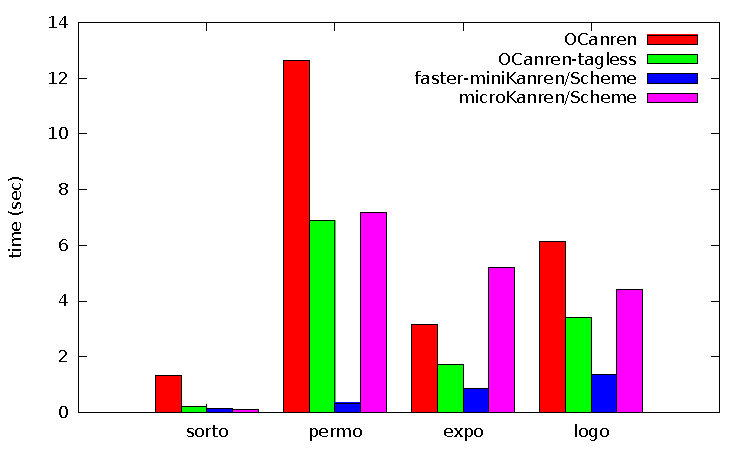
\includegraphics{graph1.pdf}
\caption{The First Set of Benchmarks}
\label{eval:first}
\end{figure}

\begin{figure}[h]
\centering
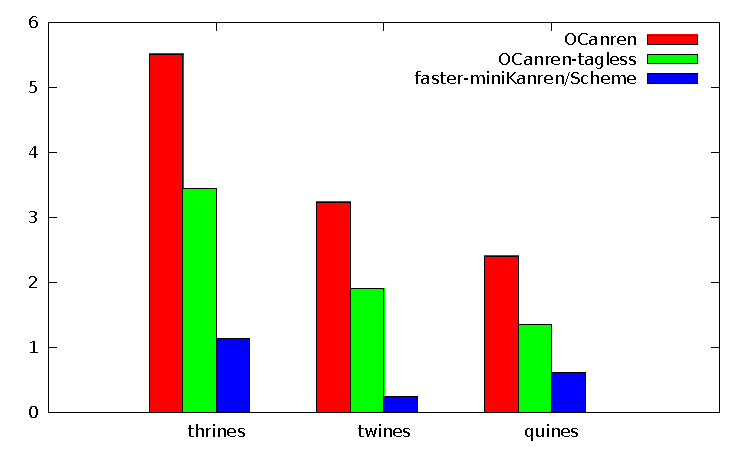
\includegraphics{graph2.pdf}
\caption{The Second Set of Benchmarks}
\label{eval:second}
\end{figure}

\section{Related Works}
\label{sec:related_works}

The non-commutativity of conjunction evaluation in miniKanren is a well-known problem. In~\cite{WillThesis} some language
extensions are discussed, which, presumably, can be used to provide the commutativity. They include both simple enumeration
of conjunct orders and more advanced techniques, based on a combination of tabling, parallel goal evaluation, and continuations.
However, by now none of these proposals were implemented or evaluated. The tabling technique, described in the same work, can
indeed be used to provide the convergence of some queries, but it deals with the problems, orthogonal to the non-commutativity,
and, thus, does not heal the queries, which we do (but heals some other cases, like divergence of path-finding queries for
graphs with cycles, which we do not). 

For a number of problems some \emph{ad-hoc} refutationally complete solutions were already presented before. For example,
in~\cite{TRS} a number of relations for binary arithmetics, implemented using the idea of bounding the sizes of terms, are
presented. In a follow-up paper~\cite{KiselyovArithmetic} this technique is explained in details, and the proof of refutational
completeness is given. Unfortunately, the specifications, written using this technique, are verbose and
hard to understand, and the implementation requires insight. Our improvement, on the other hand, makes it possible to stick
with the simplest definitions, and althought we do not provide a proof of refutational completeness for each case, for the
majority of realistic queries they converge and demonstrate the same performance, as those, implemented with advanced methods.

In a broader context of logical programming the problem of search convergence/termination was addressed multiple
times. However, it is rather hard to establish a direct correspondence between our proposal and the reported results,
since they were developed for essentially different language. For example, in~\cite{OLDresolution} a tabling-based
improvement of a resolution-based search~--- OLDT resolution~--- is described, and a complete search strategy is developed.
However, in miniKanren the original search is already complete, and we address rather a different issue. We can speculate,
that OLDT resolution roughly corresponds to the miniKanren with tabling and, thus, posesses the same properties, and relates to
our proposal in a similar manner.



\section{Conclusion}

We presented a strongly-typed implementation of \miniKanren for OCaml. Our implementation
passes all tests written for \miniKanren (including those for disequality constraints);
in addition we implemented many interesting relational programs known from
the literature. We claim that our implementation can be used both as a convenient
relational DSL for OCaml and an experimental framework for future research in the area of
relational programming.

%We also want to express our gratitude to William Byrd, who infected us with relational programming,
%and for the extra time he sacrificed as both our tutor and friend.


\bibliographystyle{ACM-Reference-Format}
\bibliography{fair-conj}

\end{document}
\endinput
%%
%% End of file `sample-sigplan.tex'.
